\section{Bunching and the elasticity of taxable income in Chile}

Taxes change behaviour, and the size of that change determines how much revenue a reform actually raises and how much welfare it costs. A schedule with an exempt threshold offers a sharp test of this mechanism: at the threshold the marginal rate rises from zero to a positive value, so taxpayers located just below it face a clear incentive to report exactly the threshold and no more. If enough of them do, the income distribution shows an abnormal pile-up at that point instead of a smooth decline. This section exploits that pile-up for the Chilean personal income tax, where the first bracket starts with a 4\% marginal rate. We ask how much of the observed concentration reflects a genuine change in declared income rather than an artefact of reporting, and we translate the answer into a single local measure of responsiveness that can be used to evaluate the revenue and efficiency consequences of moving the exemption threshold.

\textit{Bunching} is the anomalous accumulation of taxpayers at a point of the income distribution, immediately before a change in the tax schedule.  \marginnote{Bunching is the anomalous accumulation of taxpayers at a point of the income distribution}ts origin is a \textit{kink}, that is, a point where the marginal rate jumps (here from $\tau_0=0$ to $\tau_1=0.04$) without a discontinuity in the level of tax: every peso below the threshold is exempt and every peso above it is taxed at 4\%. Faced with that jump, part of the taxpayers reduce their income down to the threshold and stop locating where they would be in the absence of the rate change. That displaced mass leaves two footprints in the distribution: excess mass just below the threshold and a mass deficit just above it. When the discontinuity is in the level of tax and not in the slope, the point is called a \textit{notch}; the case analyzed here is a \textit{kink}. Figure~\ref{fig:kink_notch} shows a visual example of both cases.

\begin{figure}[htbp]
\centering
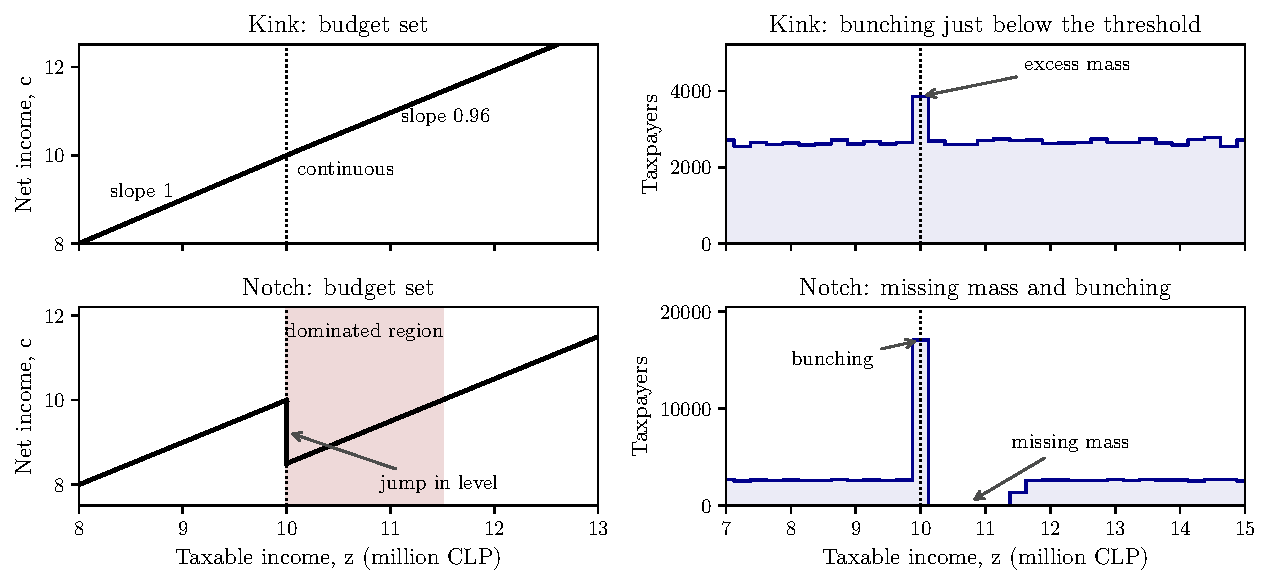
\includegraphics[width=\textwidth]{examples/kink_vs_notch.pdf}
\caption{Kink versus notch. Top row: a kink raises the marginal rate at $z^*$ without a discontinuity in net income, so taxpayers bunch just below $z^*$ and the upper branch of the budget set starts at $z^*$. Bottom row: a notch lowers net income by a fixed amount $T$ at $z^*$, which makes the interval $(z^*,\; z^*+T)$ dominated; its mass piles up at $z^*$ and the interval is left empty. Simulated with a quasilinear economy and uniformly distributed ability; income in million CLP.}
\label{fig:kink_notch}
\end{figure}

When measuring the behavioral response \marginnote{Behavioral response refers to the active re-optimization of choices by agents in response to changes in tax incentives, which alters the tax base.}to a rise in taxes we try to detect how much declared income changes when the net-of-tax rate changes, and how much of that change is a genuine response rather than an accounting artifactz The behavioral response is the change in the taxable income that taxpayers choose---hours worked, effort, bargaining over pay, deductions claimed, and the timing or legal form of income---in reaction to the tax schedule; it is what remains once the mechanical effect of the reform, namely the change in revenue holding behavior fixed, is set aside.\marginnote{The mechanical effect refers to the direct revenue change resulting from a tax reform if the tax base remained fixed at its pre-reform level.}

The elasticity of taxable income (ETI), $\epsilon$, summarizes that response as the percentage change in declared taxable income per percentage change in the net-of-tax rate $(1-\tau)$. It is an equilibrium, reduced-form parameter: it aggregates real labor supply, wage responses, shifting of income across bases and periods, and avoidance, so it exceeds the compensated labor supply elasticity and is the relevant statistic for deadweight loss, revenue feedback and optimal top rates. Bunching identifies it locally, from the taxpayers who actually relocate at the kink \parencite{chetty2011adjustment}.

\subsection{Modeling Bunching}\label{sec:modeling_bunching}
Identification combines two assumptions. First, in the absence of the \textit{kink} \marginnote{A kink is a discrete change in the slope of a choice set (such as a jump in the marginal tax rate at a bracket threshold) that leaves the budget constraint continuous.} the income density would be smooth around the threshold; for that reason a polynomial is fitted to the bins away from the \textit{kink} and projected onto the excluded region, yielding the counterfactual density $g(z)$. Second, individuals differ only in ability, with no frictions or adjustment costs, so that the mass shifting to the threshold is measurable. The excess mass $B$ is normalized by the height of the counterfactual at the threshold, $b=B/g(z^*)$, and is transformed into an elasticity through\footnote{Interpreting $\epsilon$ as a structural parameter further requires: (i) \emph{quasilinear isoelastic preferences}, ruling out income effects and imposing a common local elasticity; (ii) \emph{locally uniform density} $g(z)$ over the bunching band; (iii) \emph{no reference-point effects} at $z^*$; and (iv) a \emph{small tax jump} ($\Delta z^*/z^* \approx 0$) for the linear log approximation.}
\begin{equation}\label{eq:elasticity}
\epsilon = \frac{b}{z^* \ln\left(\dfrac{1-\tau_0}{1-\tau_1}\right)}.
\end{equation}
Equation \ref{eq:elasticity} follows from a first-order Taylor expansion of the taxpayer's optimality condition around $\ln\left(\frac{1-\tau_0}{1-\tau_1}\right)=0$. The elasticity so defined is local: it describes the response in the neighborhood of the threshold and not an arbitrary change in the rate. The same expression is derived from the taxpayer's optimality condition in Appendix~A, Equation~\ref{eq:app_final}.

\subsection{Chilean Case}
To estimate the behavioral response in Chile, we follow \cite{gutierrezNoExemption} and use administrative income-tax records from the Servicio de Impuestos Internos (SII) for dependent wage earners (\texttt{data/bunch\_counts\_wages.csv}), aggregated into annual taxable-income bins of \$100,000 CLP (\texttt{group\_0}) with taxpayer counts per bin (\texttt{NREG}). Table~\ref{tab:desc_stats} summarizes the full administrative dataset, which spans 23,926 bin-year observations across 2005--2023 with no missing entries, covering taxable incomes up to \$159.9 million CLP and an average bin count of 1,129 taxpayers (peaking at 17,707 taxpayers in a single bin). Focusing on wage earners is central to the identification design because third-party payroll withholding generates a clean observed distribution around the statutory schedule.

\begin{table}[H]
\centering
\caption{Descriptive statistics of the SII binned wage-earner dataset (2005--2023)}
\label{tab:desc_stats}
\small
\begin{adjustbox}{max width=\textwidth}
\begin{tabular}{lrrrrrrrrr}
\toprule
Variable & Count & Mean & SD & Min & P25 & Median & P75 & Max & Missing \\
\midrule
\texttt{group\_0} & 23,926 & 67.27 & 42.24 & 0.00 & 31.80 & 63.30 & 98.40 & 159.90 & 0 \\
\texttt{year} & 23,926 & 2015.27 & 5.24 & 2005 & 2011 & 2016 & 2020 & 2023 & 0 \\
\texttt{NREG} & 23,926 & 1,129.13 & 2,563.78 & 11 & 34 & 135 & 754 & 17,707 & 0 \\
\bottomrule
\end{tabular}
\end{adjustbox}
\begin{minipage}{\textwidth}
\vspace{4pt}
\footnotesize\textit{Note:} Summary statistics computed over all 23,926 bin-year observations. \texttt{group\_0} denotes the lower edge of each \$100,000 CLP taxable-income bin (rescaled to millions of CLP for readability), and \texttt{NREG} denotes the number of dependent taxpayers recorded in that bin.
\end{minipage}
\end{table}

\subsubsection*{(i) Observed distribution and first threshold}
Although the SII dataset covers 2005--2023, the raw bin counts cannot simply be pooled across all available years. Because Chile's income tax brackets are indexed in nominal terms, the statutory exemption cutoff shifts upward every year in CLP (see Figure~\ref{fig:cutoff-shift}); stacking unadjusted counts from different years would place each year's bunching spike into a different \$100,000 CLP bin and smear out the local pile-up.

\begin{figure}[H]
\centering
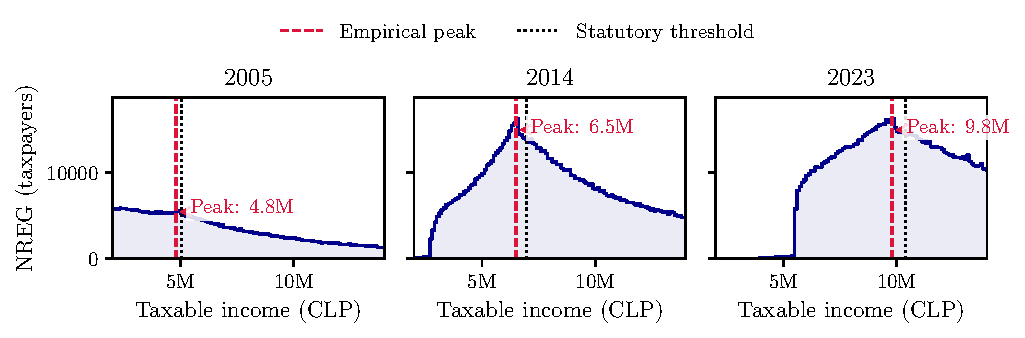
\includegraphics[width=\textwidth]{p1/p1_cutoff_shift_grid.pdf}
\caption{Nominal upward shift of the first income tax kink across selected years (2005, 2014, and 2023). Each panel displays the observed taxpayer counts (\texttt{NREG}) in \$100,000 CLP bins over a common \$2--\$14 million CLP window, alongside the empirical peak (dashed red) and the statutory exemption threshold (dotted black).}
\label{fig:cutoff-shift}
\end{figure}


Following \cite{gutierrezNoExemption}, the baseline analysis therefore focuses on the 2023 cross-section. Under Chile's personal income tax schedule (\emph{Impuesto \'Unico de Segunda Categor\'ia}), workers below the first kink face a zero marginal tax rate ($\tau_0 = 0$), whereas earnings immediately above enter the first positive bracket at $\tau_1 = 0.04$, creating a convex kink at the cutoff (located at $K = \$9{,}907{,}434$ CLP in the paper's benchmark, with the observed 2023 density peaking at \$9.8 million CLP).

Figure~\ref{fig:p1_observed} presents the observed distribution of taxable income of wage earners in 2023, constructed with \$100,000 CLP bins. 
\begin{figure}[H]
\centering
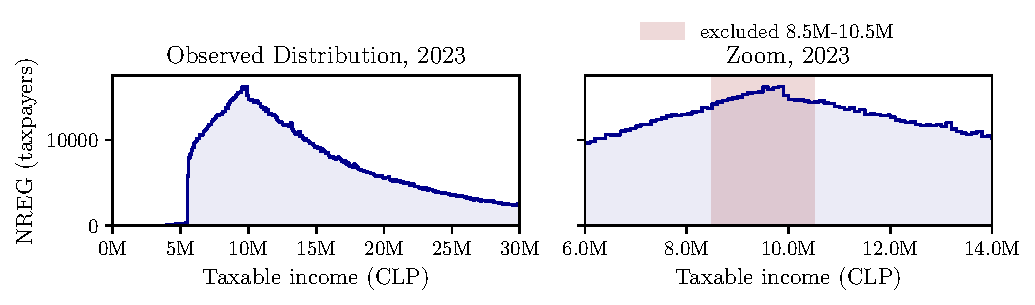
\includegraphics[width=\textwidth]{p1_observed_2023.pdf}
\caption{Observed distribution of taxable income, 2023. Left panel: full distribution; right panel: zoom between \$6 and \$14 million with the excluded region shaded.}
\label{fig:p1_observed}
\end{figure}
The number of taxpayers per bin (\texttt{NREG}) decreases monotonically with income, with an accumulation between \$9.4 and \$9.9 million and a local maximum at \$9.8 million, where 16,248 taxpayers are recorded. In the immediately higher bin, \$9.9 million, the count falls to 15,199, a reduction of 6.5\%. 

Neighboring bins confirm the profile and rule out a single-bin artefact. Averaged over the five bins that end at the peak (\$9.4--\$9.8 million) the count is 16,012 taxpayers, while over the five bins immediately above it (\$9.9--\$10.3 million) it is 14,790, a fall of 1,222 taxpayers, about 7.6\%. The deficit is not reversed in the following bins, which is the signature of mass displaced from above the threshold to the threshold itself (Figure~\ref{fig:p1_kink_neighbourhood}).

\begin{figure}[H]
\centering
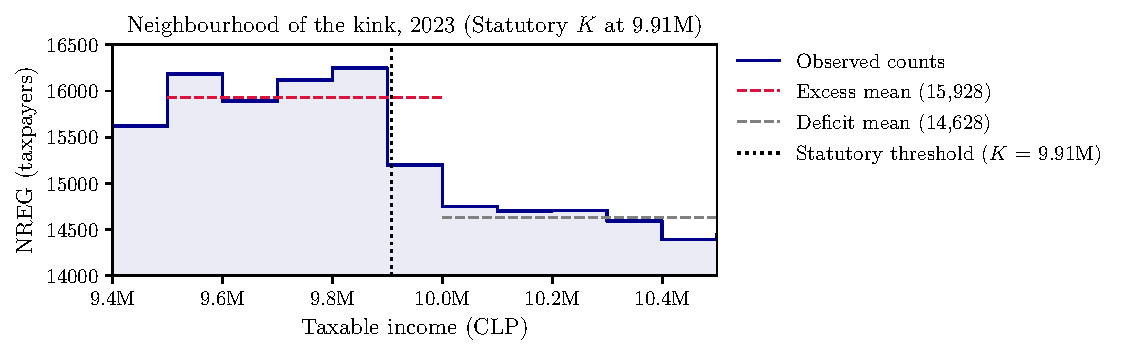
\includegraphics[width=0.95\textwidth]{p1/p1_kink_neighbourhood.pdf}
\caption{Neighbourhood of the kink, 2023. Counts of taxpayers in \$100,000 CLP bins around the peak. The dashed segments are the average count of the five bins below the peak (crimson) and of the five bins above it (grey); the dotted vertical line marks the peak.}
\label{fig:p1_kink_neighbourhood}
\end{figure}

This pattern places the empirical kink inside the \$9.8--\$9.9 million range.\footnote{The empirical location is bounded rather than pinpointed by the binned counts alone. The pile-up spans roughly \$9.4--\$9.8 million, wider than a point mass in \$100,000 bins, which reflects partial optimization frictions and income lumpiness; all of these bins lie below the cutoff, whereas a threshold at \$9.5 million would place the peak above the kink, contradicting the theoretical prediction of a deficit.} Following \cite{gutierrezNoExemption}, we set the kink at the statutory 2023 annual exemption threshold of $z^* = K = \$9{,}907{,}434$ CLP, which corresponds to the legal cutoff separating the zero-rate exempt bracket ($t_1 = 0$) from the first positive marginal tax bracket ($t_2 = 0.04$) in the 2023 tax schedule. As shown in Figure~\ref{fig:p1_kink_neighbourhood}, this statutory cutoff aligns tightly with the observed discontinuity: taxpayers accumulate immediately to the left of $K$ (peaking in the \$9.8--\$9.9 million bin) and drop sharply in the \$9.9--\$10.0 million bin just above it.


\subsubsection*{(ii) Counterfactual distribution and iterative fitting}

Let $c_j$ be the observed number of taxpayers in bin $j$, with lower limit $z_j$ and width $\Delta z$, and $\hat{c}_j$ its counterfactual value. Income is rescaled as $u_j = z_j/z_r$, where $z_r = \$20$ million is the right end of the fitting window and $[z_l, z_r]$ the window over which the polynomial is estimated. The rescaling is linear, so the fitted values do not depend on the choice of $z_r$: it only conditions the polynomial numerically.\footnote{The rescaling carries no economic content: a linear change of basis leaves the fitted values unchanged, since $a + b\,u = a + (b/z_r)\,z$ for any $z_r$, and only the coefficients are re-expressed. It is done for numerical reasons. With income in pesos, $z_j$ is of order $10^{7}$ and $z_j^{4}$ of order $10^{28}$, so the design matrix is badly conditioned and the least-squares solution loses precision; after dividing by $z_r$ the regressors lie between roughly $0.3$ and $1$ and their powers stay of order one.} A fourth-degree polynomial in $u_j$ is fitted over the \$6.5--\$20 million window, excluding the \$8.5--\$10.5 million region contaminated by the response to the kink. 

To prevent upward bias in the estimated excess mass $\hat{B}$, we implement the iterative reweighting algorithm developed by \cite{chetty2011salience}, which accounts for the ``missing mass'' above the threshold.\footnote{\texttt{code: source/bunching/model.py:L5}} Because taxpayers who bunch at $z^*$ originate from the upper tail, the observed density to the right of the excluded region is depressed relative to the true counterfactual. The iterative procedure is summarized in Algorithm~\ref{alg:p1_iter}, where observed counts outside the excluded region and right tail are iteratively scaled upwards based on the estimated bunching mass until convergence.

\begin{algorithm}[H]
\caption{Iterative estimation of the counterfactual density with Chetty et al. (2011) reweighting}
\label{alg:p1_iter}
\begingroup
\renewcommand{\baselinestretch}{1.25}\selectfont
\begin{algorithmic}[1]
\Require bin edges $z_j$, counts $c_j$, fitting window $[z_l, z_r]$, excluded region $[z_L, z_R)$, degree $p$, tolerance $\text{tol}$
\Ensure counterfactual counts $\hat{c}_j$ for every bin in the window
\State $u_j \gets z_j / z_r$ \Comment{rescaling for numerical conditioning}
\State $P_p(u; \beta) \equiv \sum_{i=0}^{p} \beta_i u^i$ \Comment{degree-$p$ polynomial in rescaled income}
\State $\mathcal{A} \gets \{j : z_l \le z_j \le z_r\}$ \Comment{fitting window}
\State $\mathcal{E} \gets \{j : z_L \le z_j < z_R\}$ \Comment{excluded bunching region}
\State $\mathcal{R} \gets \{j : z_R \le z_j \le z_r\}$ \Comment{right-side tail to be reweighted}
\State $c^{(0)}_j \gets c_j$ for all $j$, \quad $M_R \gets \sum_{j \in \mathcal{R}} c_j$ \Comment{initialize counts and right-tail mass}
\For{$k = 1, 2, \dots$}
    \State fit $P_p(u;\beta)$ by least squares to $c^{(k-1)}_j$ over $j \in \mathcal{A} \setminus \mathcal{E}$, giving $\hat{\beta}^{(k)}$ \Comment{fit on clean bins}
    \State $\hat{c}^{(k)}_j \gets P_p(u_j;\hat{\beta}^{(k)})$ \quad for all $j \in \mathcal{A}$ \Comment{predicted counterfactual}
    \State $\hat{B}^{(k)} \gets \sum_{j \in \mathcal{E}} \left( c_j - \hat{c}^{(k)}_j \right)$ \Comment{estimate excess bunching mass}
    \State $c^{(k)}_j \gets c_j \left(1 + \frac{\hat{B}^{(k)}}{M_R}\right)$ for $j \in \mathcal{R}$, \quad $c^{(k)}_j \gets c_j$ otherwise \Comment{reweight right tail}
    \If{$\max_{j \in \mathcal{R}} \left| c^{(k)}_j - c^{(k-1)}_j \right| < \text{tol}$}
        \State \textbf{break}
    \EndIf
\EndFor
\State \Return $\hat{c}_j \equiv \hat{c}^{(K)}_j$ \Comment{$K$ = last completed iteration}
\end{algorithmic}
\endgroup
\end{algorithm}

The iteration is necessary because a single fit on the unadjusted distribution extrapolates a curve pulled downward by the depressed right tail, underestimating the counterfactual density around the threshold and inflating the estimated excess mass $\hat{B}$. By iteratively scaling up the right tail to account for the missing mass, the polynomial converges to the true counterfactual distribution on both sides of the cutoff. Figure~\ref{fig:p1_counterfactual} compares the observed and converged counterfactual distributions, while Figure~\ref{fig:p1_chetty_comparison} isolates the quantitative impact of the right-tail reweighting correction relative to the unadjusted one-step polynomial fit.

\begin{figure}[htbp]
\centering
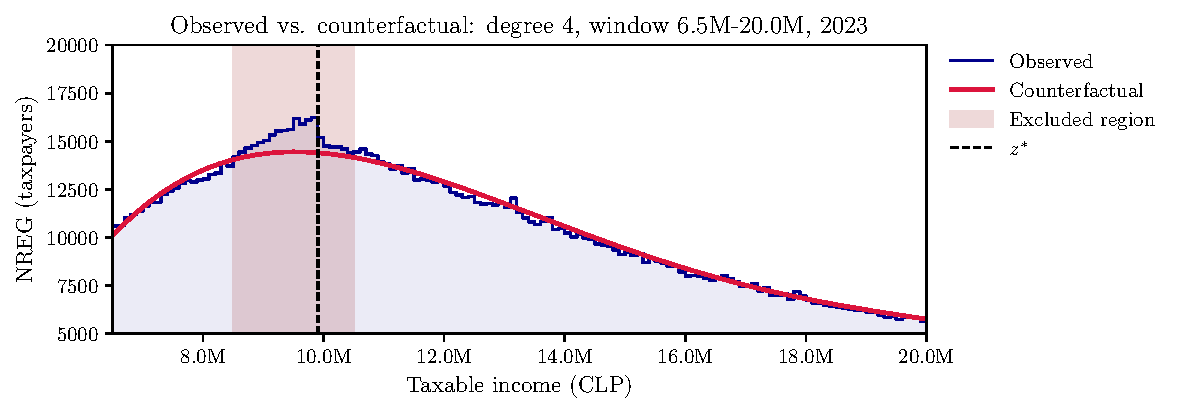
\includegraphics[width=\textwidth]{p1_counterfactual_2023.pdf}
\caption{Observed and counterfactual distribution of taxable income, 2023. The red line corresponds to the estimated counterfactual and the shaded band to the excluded region.}
\label{fig:p1_counterfactual}
\end{figure}

\begin{figure}[htbp]
\centering
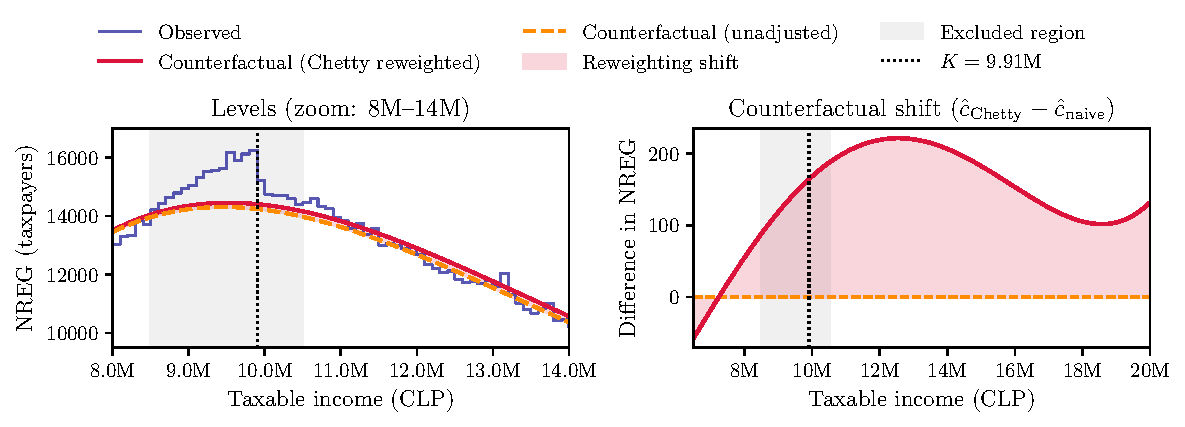
\includegraphics[width=\textwidth]{p1/p1_chetty_comparison.pdf}
\caption{Effect of iterative right-tail reweighting on the counterfactual fit, 2023. Left panel: zoomed comparison in levels between \$8 and \$14 million CLP showing the upward shift from the unadjusted one-step fit (dashed orange) to the converged Chetty et al.\ (2011) counterfactual (solid crimson). Right panel: bin-by-bin difference ($\hat{c}_{\mathrm{Chetty}} - \hat{c}_{\mathrm{naive}}$) across the full \$6.5--\$20 million CLP estimation window, illustrating how redistributing the displaced mass lifts the upper tail and corrects the downward bias near the kink $K$.}
\label{fig:p1_chetty_comparison}
\end{figure}


\subsubsection*{(iii) Excess mass and elasticity}

To operationalize the continuous identification framework of Section~\ref{sec:modeling_bunching} on binned administrative records, we approximate the counterfactual density at the threshold, $g(z^*)$, by the average counterfactual density per peso across the excluded region $\mathcal{E} = \{j : z_L \le z_j < z_R\}$,
\begin{equation}
\hat{B} = \sum_{j \in \mathcal{E}} \left(c_j - \hat{c}_j\right), \qquad 
\hat{b} = \frac{\hat{B}}{\bar{g}}, \qquad 
\bar{g} = \frac{1}{N_{\mathcal{E}}\,\Delta z}\sum_{j \in \mathcal{E}} \hat{c}_j,
\end{equation}
where $N_{\mathcal{E}} = 20$ is the number of $\Delta z = \$100{,}000$ CLP bins in $[8.5\text{M}, 10.5\text{M})$ and $\hat{b}$ recovers the empirical counterpart of the behavioral income shift $\Delta z^*$ in CLP. Substituting $\hat{b}$ and the 2023 statutory parameters ($z^* = K = \$9{,}907{,}434$ CLP, $\tau_0 = 0$, and $\tau_1 = 0.04$, so that $\ln[(1-\tau_0)/(1-\tau_1)] \approx 0.04082$) directly into Equation~\eqref{eq:elasticity} yields the local taxable-income elasticity $\hat{\epsilon}_E$.

Under the baseline specification with right-tail reweighting, we obtain an excess mass of $\hat{B} = 16{,}219.3$ taxpayers, corresponding to a normalized behavioral response of $\hat{b} = \$113{,}160$ CLP under \textit{mean} normalization and $\hat{b} = \$115{,}456$ CLP under \textit{kink} normalization. Evaluated at the statutory threshold $K = \$9{,}907{,}434$ CLP, the \textit{mean}-normalized estimate delivers $\hat{\epsilon}_E = 0.2799$ ($\hat{\epsilon} = 0.2856$ under \textit{kink} normalization), reproducing the benchmark elasticity reported by \cite{gutierrezNoExemption} to four decimal places.\footnote{\texttt{code: source/bunching/model.py:L170}}

Because the excluded region $[8.5\text{M}, 10.5\text{M})$ is held fixed, $\hat{B}$ and $\hat{b}$ remain invariant to local perturbations of the threshold location, while $\hat{\epsilon}$ varies inversely with $z^*$. Varying $z^* \in \{\$9.6, \$9.8, \$9.91, \$10.0, \$10.4\}$ million CLP across both normalization rules bounds the elasticity within the narrow interval $[0.2665, 0.2946]$. Moreover, switching from \textit{mean} to \textit{kink} normalization shifts $\hat{\epsilon}$ by less than $0.006$ across every cutoff, confirming that the counterfactual density is nearly uniform across the bunching band and that the estimated behavioral response is robust to local normalization choices.

Figure~\ref{fig:p1_sensitivity} illustrates the sensitivity grid across candidate thresholds and normalization rules, highlighting the narrow stability band around the statutory benchmark.

\begin{figure}[htb!]
\centering
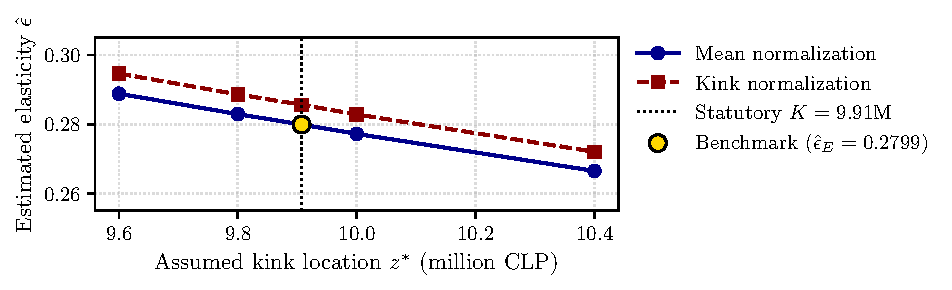
\includegraphics[width=0.85\textwidth]{p1/p1_elasticity_sensitivity.pdf}
\caption{Sensitivity of $\hat{\epsilon}$ to the assumed kink $z^*$ and normalization rule (\textit{mean} vs.\ \textit{kink}), 2023. The dotted line and marker denote the statutory threshold $K = \$9.91$M CLP and benchmark $\hat{\epsilon}_E = 0.2799$ \parencite{gutierrezNoExemption}.}
\label{fig:p1_sensitivity}
\end{figure}

\subsubsection*{(iv) Sensitivity}

Table~\ref{tab:p1_iv} and Figure~\ref{fig:p1_iv} summarize 16 specifications\footnote{\texttt{code: scripts/make\_p1\_iv\_table.py:L23}} combining four bin widths ($\Delta z \in \{\$100{,}000,\; \$200{,}000,\; \$300{,}000,\; \$500{,}000\}$ CLP) with four estimation windows ($[z_l, z_r] \in \{[\$6.5\text{M}, \$20\text{M}],\; [\$5\text{M}, \$20\text{M}],\; [\$6.5\text{M}, \$30\text{M}],\; [\$5\text{M}, \$30\text{M}]\}$), holding fixed the fourth-degree polynomial specification, the excluded bunching region $[\$8.5\text{M}, \$10.5\text{M})$, the statutory 2023 exemption cutoff $K = \$9{,}907{,}434$ CLP, and the iterative right-tail reweighting procedure.

\begin{table}[htbp]
\centering
\small
\begin{tabular}{rrrrr}
\toprule
Bin (thousand CLP) & Window (CLP) & $B$ & $b$ (CLP) & $\hat\epsilon$ \\
\midrule
100 & 6.5-20.0M & 20\,089.6 & 141\,932 & 0.355 \\
100 & 5.0-20.0M & 8\,996.4 & 61\,272 & 0.153 \\
100 & 6.5-30.0M & 34\,773.2 & 258\,437 & 0.646 \\
100 & 5.0-30.0M & 27\,750.3 & 201\,241 & 0.503 \\
200 & 6.5-20.0M & 18\,993.2 & 133\,696 & 0.334 \\
200 & 5.0-20.0M & 9\,620.1 & 65\,554 & 0.164 \\
200 & 6.5-30.0M & 33\,514.2 & 248\,617 & 0.622 \\
200 & 5.0-30.0M & 26\,732.6 & 193\,444 & 0.483 \\
300 & 6.5-20.0M & 20\,559.5 & 145\,347 & 0.363 \\
300 & 5.0-20.0M & 11\,895.6 & 81\,714 & 0.204 \\
300 & 6.5-30.0M & 35\,872.0 & 267\,383 & 0.668 \\
300 & 5.0-30.0M & 28\,581.1 & 207\,664 & 0.519 \\
500 & 6.5-20.0M & 18\,389.5 & 129\,242 & 0.323 \\
500 & 5.0-20.0M & 16\,154.0 & 112\,646 & 0.282 \\
500 & 6.5-30.0M & 33\,722.3 & 250\,498 & 0.626 \\
500 & 5.0-30.0M & 30\,065.8 & 220\,344 & 0.551 \\
\bottomrule
\end{tabular}
\caption{Estimated elasticity by bin width and estimation window.}
\label{tab:p1_iv}
\end{table}


Across all 16 specifications, $\hat{\epsilon}$ remains strictly positive, spanning the interval $[0.1272,\, 0.5271]$, while the excess mass $\hat{B}$ ranges between $7{,}596.5$ and $29{,}175.4$ taxpayers. Comparing both dimensions reveals a clear asymmetry in how tuning choices affect the estimator:
\begin{enumerate}
    \item \textbf{Stability with respect to bin width ($\Delta z$):} Holding the baseline estimation window fixed at $\$6.5$--$\$20$ million CLP, varying $\Delta z$ across $\$100{,}000$, $\$200{,}000$, $\$300{,}000$, and $\$500{,}000$ CLP yields elasticities of $0.2798$, $0.2584$, $0.2564$, and $0.2163$, respectively. For bin widths up to $\$300{,}000$ CLP, the estimates stay tightly clustered within $[0.2564,\, 0.2798]$ around the benchmark $\hat{\epsilon}_E = 0.2799$ \parencite{gutierrezNoExemption}, with a modest attenuation only at $\Delta z = \$500{,}000$ CLP where coarse aggregation ($4$ excluded bins) smooths out the sharp peak immediately below $K$.
    \item \textbf{Dominance of the estimation window ($[z_l, z_r]$):} Holding $\Delta z = \$100{,}000$ CLP fixed and shifting the outer bounds of the fitting window produces much wider variation: $\hat{\epsilon}$ falls to $0.1272$ under $\$5$--$\$20$ million CLP, rises to $0.5271$ under $\$6.5$--$\$30$ million CLP, and reaches $0.4232$ under $\$5$--$\$30$ million CLP. Because a fourth-degree polynomial is extrapolated across the excluded band $[\$8.5\text{M}, \$10.5\text{M})$, extending the right tail to $\$30$ million or lowering the left cutoff to $\$5$ million alters the global curvature of the counterfactual and shifts the baseline density height $\bar{g}$ around $K$.
\end{enumerate}

Thus, while every specification confirms a positive behavioral response at Chile's first income tax kink, the sensitivity to the fitting window highlights that polynomial bunching estimates are local approximations whose point magnitude depends on the outer bounds used to discipline counterfactual curvature. Appendix~\ref{app:pooled_bunching} explores whether pooling observations across all available years (2005--2023) after normalizing by each year's statutory threshold or empirical mode mitigates finite-sample noise in this local estimation.

\begin{figure}[htbp]
\centering
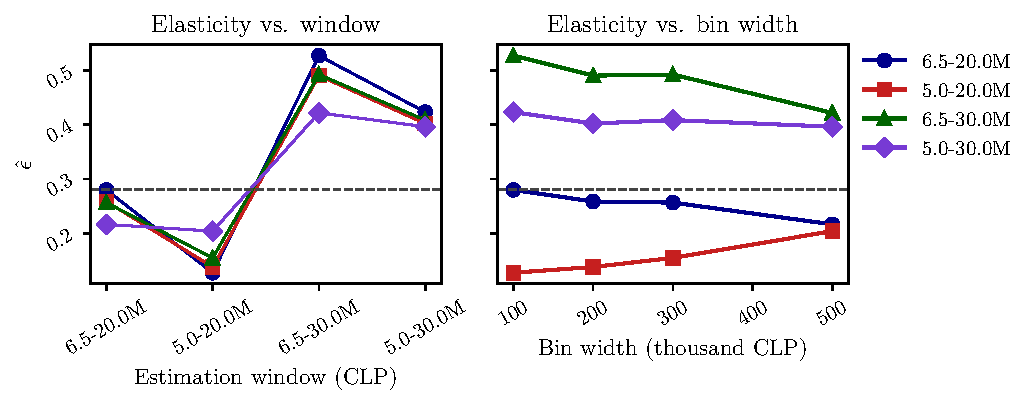
\includegraphics[width=\textwidth]{p1_iv_sensitivity.pdf}
\caption{Sensitivity of the estimated taxable-income elasticity $\hat{\epsilon}$ across bin widths and estimation windows, 2023. Left panel: $\hat{\epsilon}$ by estimation window, one line per bin width. Right panel: $\hat{\epsilon}$ by bin width, one line per estimation window. The dashed gray line marks the benchmark estimate $\hat{\epsilon}_E = 0.2799$.}
\label{fig:p1_iv}
\end{figure}

\subsubsection*{(v) Economic interpretation}

Under the standard isoelastic bunching framework, the benchmark estimate $\hat{\epsilon}_E = 0.2799$ ($\hat{\epsilon} = 0.2856$ under \textit{kink} normalization) implies that a $1\%$ decrease in the net-of-tax rate $(1-\tau)$ reduces declared taxable income by $0.28\%$ in the neighborhood of Chile's first statutory bracket cutoff ($K = \$9{,}907{,}434$ CLP, where $\tau$ rises from $0$ to $0.04$). In monetary terms, this corresponds to an average income compression of $\hat{b} = \$113{,}160$ CLP per year ($\approx 1.14\%$ of $K$) and an excess mass of $\hat{B} = 16{,}219.3$ taxpayers in 2023.

To evaluate how this estimate informs a policy proposal to lower the personal income tax exemption threshold, $\hat{\epsilon}_E$ must be placed within the mechanical--behavioral decomposition of base-broadening reforms \parencite{gutierrezNoExemption}. Lowering the exemption threshold has an asymmetric incidence: the mechanical revenue gain falls broadly across \emph{all} formal wage earners located above the new cutoff, whereas intensive-margin behavioral leakage is concentrated locally near the threshold where taxpayers transition from the $0\%$ to the $4\%$ bracket. Because the first marginal rate in Chile is low ($\tau_1 = 0.04$), the associated net-of-tax wedge $\frac{\tau_1}{1-\tau_1} \approx 0.0417$ is exceptionally small; scaled by $\hat{\epsilon}_E = 0.2799$, intensive-margin behavioral responses erode only about $1.17\%$ of each marginal peso taxed at the first bracket.

However, treating $\hat{\epsilon}_E \approx 0.28$ as a deep, policy-invariant labor-supply elasticity---or invoking low intensive-margin leakage to justify base broadening from below as an efficient fiscal solution---warrants four substantive caveats rooted in bunching theory and Chilean institutional reality:

\begin{enumerate}
    \item \textbf{Compensation packaging vs.\ structural labor supply under adjustment frictions:} In the benchmark international literature, dependent wage earners subject to third-party payroll withholding display near-zero bunching ($\epsilon \approx 0$), with excess mass concentrated among self-employed filers who control income reporting \parencite{saez2010taxpayers,saez2012elasticity}. Moreover, theoretical models with fixed adjustment costs show that optimization frictions severely attenuate observed bunching at small kinks ($\Delta\tau = 0.04$), because the utility gain from re-optimizing scales quadratically in $(\Delta\tau)^2$ \parencite{chetty2011adjustment}. Finding $\hat{\epsilon}_E \approx 0.28$ alongside a diffuse pile-up across $\$9.4$--$\$9.8$ million CLP (Figure~\ref{fig:p1_kink_neighbourhood}) therefore points away from frictionless adjustments in hours worked. Instead, it reflects firm-level compensation design and statutory packaging around a salient annual threshold---specifically, the use of tax-exempt allowances (\textit{asignaciones} for mobilization, meals, or per diems), discretionary year-end bonuses, and payment timing that allow employers and workers to target net take-home pay just below $K$ at low adjustment cost.

    \item \textbf{Non-parametric non-identification and sensitivity to counterfactual curvature:} As demonstrated in Section~(iv), varying the outer polynomial fitting window shifts $\hat{\epsilon}$ across $[0.1272,\, 0.5271]$---a fourfold span that conventional standard errors from a single specification conceal. This instability illustrates the fundamental identification result of \textcite{blomquist2021bunching}: with a single cross-sectional kink and no exogenous variation in tax rates, the taxable-income elasticity is not non-parametrically identified without untestable functional-form restrictions on the counterfactual density $g(z)$ inside the excluded band.

    \item \textbf{Unobserved extensive-margin informality and cross-base spillovers:} Bunching at $K$ identifies solely an \emph{intensive-margin} response among workers who remain inside the formal SII registry. Lowering the exemption threshold pulls lower-middle-income workers into the tax net for the first time, activating an \emph{extensive-margin} participation choice between formal payroll employment and informal self-employment or unregistered wage work. In a segmented labor market like Chile's, formalization elasticity at lower earnings can substantially exceed intensive-margin bunching, eroding revenue while weakening social-security coverage and aggregate productivity. Conversely, informal workers still remit indirect taxes (such as VAT on formal inputs), creating cross-base fiscal externalities that a single-base ETI ignores.

    \item \textbf{Limited revenue ceiling and distributional incidence in a top-concentrated economy:} Because Chile's exemption threshold sits relatively high in the formal earnings distribution---leaving roughly three-quarters of formal wage earners exempt \parencite{gutierrezNoExemption}---an annual threshold near $\$9.9$ million CLP ($\approx \$825{,}000$ CLP/month) lies around the upper quartile of formal salaries. Even so, lowering the threshold applies a flat $4\%$ rate to a narrow slice of middle- and lower-middle-income labor earnings, generating a low revenue ceiling regardless of how small intensive-margin leakage is. Meanwhile, Chile's fiscal capacity is overwhelmingly concentrated at the top, where the top $1\%$ captures $22$--$26\%$ of total income (and up to $40$--$44\%$ once accrued business profits and evasion are included; \parencite{fairfield2016top,flores2020top}) while paying low effective tax rates ($11$--$16\%$) due to corporate profit retention \parencite{bohme2022diagnostico}. Compressing the wage exemption threshold thus taxes transparent middle-class payrolls while leaving top-end capital income untouched.
\end{enumerate}

In sum, $\hat{\epsilon}_E = 0.2799$ provides a disciplined local input for quantifying intensive-margin leakage near the first kink, showing that a $4\%$ marginal rate induces modest direct tax-base erosion. Yet it should not be misread as a structural labor-supply parameter: rather than capturing neoclassical hours preferences, it reflects institutional pay-packaging around a known threshold, and it offers no substitute for addressing extensive-margin informality or taxing concentrated capital income at the top of the distribution.